\chapter{Lazy Load}

\section{Descrizione}

"An object that doesn’t contain all of the data you need but knows how to get it" - Martin Fowler

Quando una Classe deve mantenere memorizzati dei dati, e' utile che essi siano caricati tanto tardi quanto e' bassa la probabilita' che si ricorra ad essi.
Ovvero si rimanda il caricamento dei dati alla prima occorrenza di utilizzo.
Per ottenere questo e' necessario che essa possa ottenere o popolare i dati che gli spettano.

\section{Vista UML}

\begin{center}
    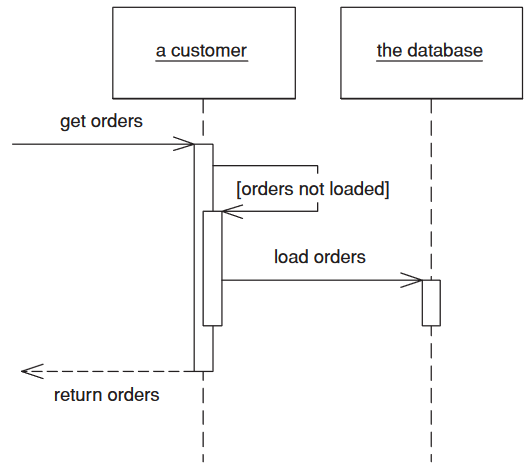
\includegraphics[width=12cm]{images/lazy-load/LazyLoad.png}
\end{center}

\section{Vantaggi}

Il vantaggio principale riguarda le prestazioni e in particolare la velocita' con cui una classe o istanza viene caricata in memoria.
Se meno dati vengono precaricati (perche' al momento inutili) allora minore sara' il carico di lavoro dei calcolatori che la elaborano.
Inoltre se l'istanza verra' eliminata dalla memoria senza che quei dati vengano acceduti, sara' possibile risparmiare anche sul tempo di eliminazione dei dati.
Bisogna altresi' considerare che questo determina anche un uso piu' ottimizzato della memoria: per tutto il tempo in cui non sara' necessaria la risorsa A, ci sara' piu' spazio in memoria per utilizzare il resto delle risorse.

\section{Svantaggi}

Si supponga ora che la classe abbia come responsabilita' la manipolazione dei dati e il caricamento lazy degli stessi.
Il Single Responsibility Principle prescrive che ogni classe abbia solo una responsabilita', in modo tale che abbia meno motivi possibili per diventare obsoleta.
Se si vuole rispettare questo principio occorre esportare la responsabilita' di caricamento lazy ad una classe di supporto.
Questo pero' genera necessariamente accoppiamento a seguito di questa nuova dipendenza.
E' quindi essenziale effettuare una scelta ponderata che tenga conto delle priorita'.

\section{Quando Usarlo}

Questa strategia e' utile quando i dati non sono immediatamente necessari per l'elaborazione e quando per recuperarli servono molteplici operazioni rimandabili.
Quando una operazione deve essere fatta e' utile caricare tutti i dati che essa possa caricare per evitare di doverla ripetere. E' quindi consigliato evitare di inserire Lazy Load multipli a meno che non si tratti di dati eterogenei e ulteriormente rimandabili.
Quando si vuole gestire dall'interno una inizializzazione onerosa e complessa e' di norma possibile applicare senza troppi problemi questo pattern per articolare questa fase senza sbilanciare il carico dell'applicativo.